\documentclass{report}

%%%%%%%%%%%%%%%%%%%%%%%%%%%%%%%%%%%%%%%%%%%%%%%%%%%%%%%%%%%%%%%%%%%%%
%                            Preamble
%%%%%%%%%%%%%%%%%%%%%%%%%%%%%%%%%%%%%%%%%%%%%%%%%%%%%%%%%%%%%%%%%%%%%%
\usepackage[utf8]{inputenc}
% Define page size and margin size
\usepackage{geometry}
\geometry{
    a4paper,
    total={170mm,257mm},
    left=20mm,
    top=20mm,
}
\usepackage{hyperref}
\usepackage{multicol}
\usepackage{wrapfig}
\usepackage[utf8]{inputenc} %to import other docs
\usepackage[DIV=14]{typearea} % to change page size on the fly
\usepackage{pgfgantt} %to insert gantt chart
\usepackage{float} %goddamn figure places
\usepackage{enumitem}
\setlength\parindent{0pt}
% reformat chapter display
\usepackage{titlesec}
\titleformat{\chapter}{\normalfont\LARGE\bfseries}{\thechapter}{1em}{\LARGE}
\titlespacing*{\chapter}{0pt}{0pt}{10pt}

\counterwithout{figure}{chapter} %global figure counter

\renewcommand{\bibname}{References}
% \renewcommand{\today}{\formatdate{10}{20}{2020}}


\begin{document}
%%%%%%%%%%%%%%%%%%%%%%%%%%%%%%%%%%%%%%%%%%%%%%%%%%%%%%%%%%%%%%%%%%%%%
%TITLE PAGE AND TABLE OF CONTENTS
%%%%%%%%%%%%%%%%%%%%%%%%%%%%%%%%%%%%%%%%%%%%%%%%%%%%%%%%%%%%%%%%%%%%%%
\begin{titlepage}
    \begin{center}
        \vspace*{1cm}

        \Huge
        \textbf{Design Plan}

        \vspace{1.5cm}
        \Large
        Modular Garden Monitoring System\\
        EECS Senior Design 2021

        \vspace{0.5cm}
        October 20, 2020

        \vspace{1.5cm}

        \textbf{Team CE12} \\
        {\Large Sadie Gladden, Eric Krenz, Zuguang Liu, Alan Trester}

        \vspace{1.5cm}
        \textbf{Technical Advisor} \\
        {\Large Dr. Zachariah Fuchs}

        \vfill

        University of Cincinnati\\
        College of Engineering and Applied Science\\
        EECE 5031 CompE Senior Design I - 001

        \vspace{0.8cm}
    \end{center}
\end{titlepage}

\tableofcontents

%%%%%%%%%%%%%%%%%%%%%%%%%%%%%%%%%%%%%%%%%%%%%%%%%%%%%%%%%%%%%%%%%%%%%%
%PROBLEM STATEMENT
%%%%%%%%%%%%%%%%%%%%%%%%%%%%%%%%%%%%%%%%%%%%%%%%%%%%%%%%%%%%%%%%%%%%%%
\chapter{Problem Statement}

Lawns and gardens are one of most essential elements for the typical American home. A survey conducted by National Association of Landscape Professionals in 2019 shows that 79 percent of American families value lawns when renting or buying a home, and about one in three Americans garden in their yards multiple times a week\cite{noauthor_new_2019}. \\

Consequently, there is a constantly high demand of water for use in lawns and garden. Per the United States Environmental Protection Agency, about 48 gallons of water is devoted for this use per family per day. Across America, nearly 1/3 of all residential water is used for landscaping irrigation totaling an estimated 9 billion gallons per day\cite{epa_outdoor_nodate}. In a world undergoing climate change with consistent annual water shortages and wildfires in many parts of the world, wasteful water usage is simply unacceptable. \\

A 21st-century solution is needed to help new homeowners care for their lawns and gardens in a more informed and effective way while reducing the amount of wasteful water usage that is accounted for by residential lawn care and irrigation. \\

Originated from the Internet of Things (IoT) concept, the Modular Garden Monitoring System (MGMS) is a solution that will be able to provide real-time and historical information about environmental conditions. Simply having detailed information on-hand will allow homeowners to make more informed decisions on the types of plants to keep in their gardens as well as when and how much to water them. Internet connectivity can take decision making to the next level by being able to crowd-source gardening recommendations and consider local weather predictions for watering. Further system expansions can introduce features such as automatic watering to take work from homeowner's shoulders while reducing human error in the garden care process. Finally, a smart design will allow the system to be flexible and applicable in a variety of scenarios varying with garden size and irrigation needs and even between residential and industrial settings.
%%%%%%%%%%%%%%%%%%%%%%%%%%%%%%%%%%%%%%%%%%%%%%%%%%%%%%%%%%%%%%%%%%%%%%
%OBJECTIVES AND CONSTRAINTS
%%%%%%%%%%%%%%%%%%%%%%%%%%%%%%%%%%%%%%%%%%%%%%%%%%%%%%%%%%%%%%%%%%%%%%
\chapter{Objectives and Constraints}

A garden monitoring system such as the one we are proposing is not a novel idea: several products already exist within the consumer and industrial farming markets with similar approaches towards data collection. The Onset HOBOnet system is a web-enabled data-collection solution for industrial farmers. While these systems are very popular and provide good results, with accessible user interfaces and informative data visualization, they are too expensive for consideration by homeowners and don’t have the necessary features such as garden suggestions to be applicable in that market \cite{onsethobo}. The Edyn Garden Sensor was a consumer-targeted system that aimed to tackle the same problems as the MGMS, unfortunately the product was burdened with limited modularity and expandability as well as a poorly designed app interface \cite{edyn}. Characteristics of both products are analyzed and, along with interviews and the team’s own expectations, are used to set a reasonable objectives baseline for the new system.

\section{Attribute Table}
Figure \ref{fig:attribute} shows a completed attribute table for the MGMS. Attributes were decided by the project team with insight from research into the products mentioned above as well as an interview of an agricultural engineering professional which helped gained insight into helpful functions and realistic expectations for system functionality. Other constraints and functions were chosen to support the proposed system goals. The most significant attributes that determines the success of the project are:

\begin{enumerate}[label=\alph*.]
    \item
          High importance placed on accuracy and accessible UIs, which are the most characteristic feature of the HOBOnet industrial system.
    \item
          Expandability and Modularity, which was identified as a shortcoming of the Edyn garden system.
    \item
          Low Cost to match the Edyn’s reasonable price tag between 75-150 per system module.\\
\end{enumerate}

\vspace{-13pt}
\begin{figure}[H]
    \centering
    \includegraphics[width=0.8\linewidth]{PNGs/AttributeTable.PNG}
    %I changed it from \linewidth only because it made the captions fit better ¯\_(ツ)_/¯
    %-- oh my b
    \caption{MGMS Attribute Table. Attributes were chosen with insight from a variety of sources including interviews and product market research.}
    \label{fig:attribute}
\end{figure}


\section{Objective Tree}

Figures \ref{fig:hw_obj} and \ref{fig:sw_obj} show expanded objective trees for the hardware and software components of the MGMS respectively. Objectives were chosen from the attribute table in figure 1. Then, main categories towards which these objectives are contributing were identified for greater organization of the project goals. These goals are:

\begin{multicols}{2}
    Hardware:
    \begin{itemize}
        \item
              Marketable
        \item
              Useful
        \item
              Reliable
    \end{itemize}
    Software:
    \begin{itemize}
        \item
              Accessible
        \item
              Customizable
        \item
              Helpful
    \end{itemize}
\end{multicols}

% \vspace{7mm} % space cause \\doesnt work here?

\begin{figure}[H]
    \centering
    \includegraphics[width=\linewidth]{PNGs/HW_Objective_Tree.PNG}
    \caption{MGMS Hardware objectives tree grouped into three component goals: Marketable, Useful, and Reliable.}
    \label{fig:hw_obj}
\end{figure}

\begin{figure}[H]
    \centering
    \includegraphics[width=\linewidth]{PNGs/SW_Objective_Tree.PNG}
    \caption{MGMS Software objectives tree grouped into three component goals: Accessible,Customizable,Helpful.}
    \label{fig:sw_obj}
\end{figure}

\section{Impact-Effort Matrix}
Impact-effort matrix is a tool that helps organize priorities so that practically limited time and resource can be used effectively. Tasks in the early stage of the project are placed in such matrix in Figure \ref{fig:impact_effort}, where it becomes obvious that meeting the basic design requirements and goals should be the first priority. It is also important to keep good documents and communications, but since it does not require much effort, a focused time slot per week should be enough investment. As far as the low-impact items, implementing ``good-to-have'' features is the last priority provided that there is still time and resource to spare, whereas features out of scope of the project will not be considered in the development at all.

\vspace{15pt}
\begin{figure}[H]
    \centering
    \begin{minipage}{0.9\linewidth}
        % Just so you guys know I'm too good to make this doable in LaTex --Liu
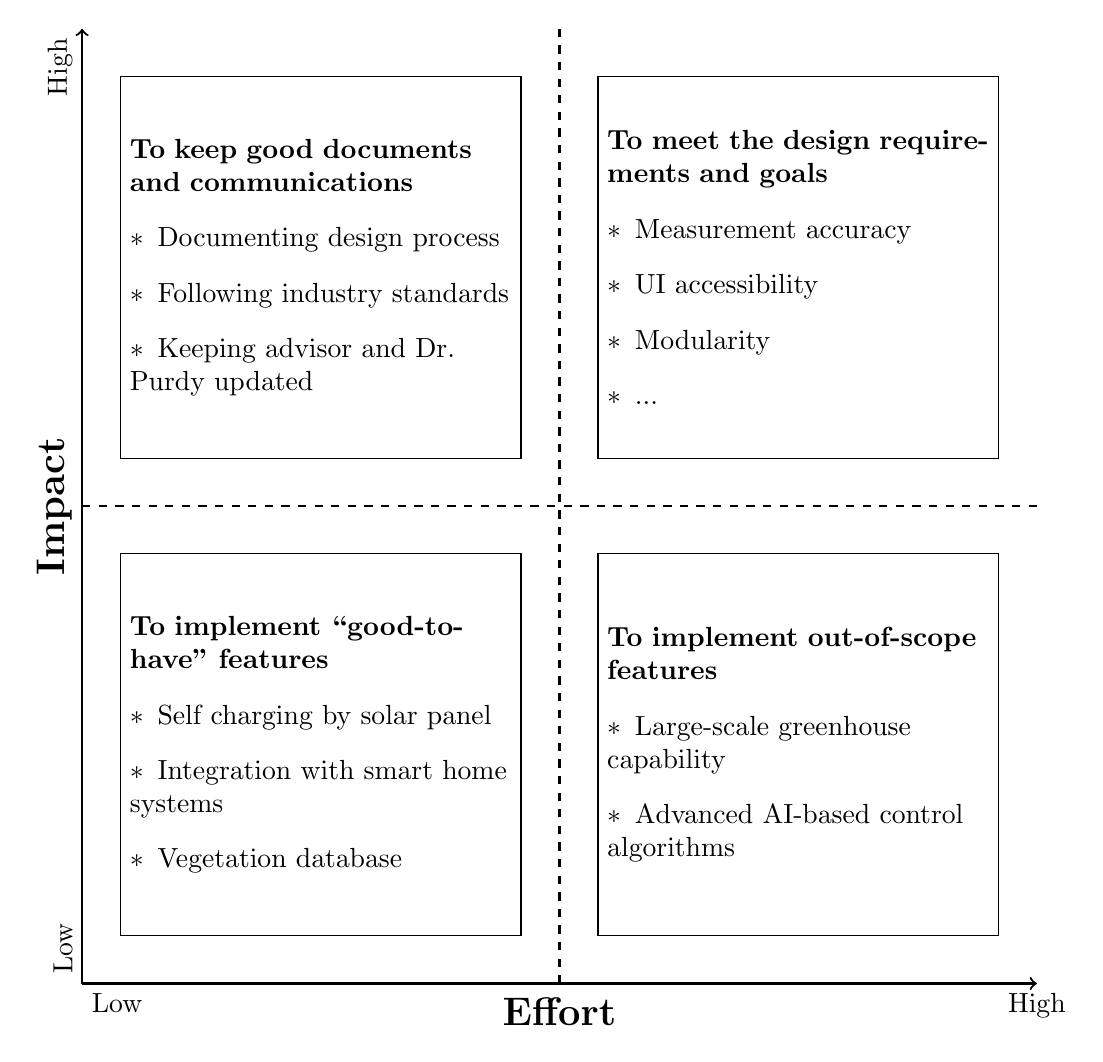
\begin{tikzpicture}
    % Axes
    \draw [thick, dashed] (-0.5\linewidth,0) -- (0.5\linewidth,0);
    \draw [thick, dashed] (0,-0.5\linewidth) -- (0,0.5\linewidth);
    \draw [thick, ->] (-0.5\linewidth,-0.5\linewidth) -- (-0.5\linewidth,0.5\linewidth);
    \draw [thick, ->] (-0.5\linewidth,-0.5\linewidth) -- (0.5\linewidth,-0.5\linewidth);
    % Labels
    \node [below right] at (-0.5\linewidth,-0.5\linewidth) {Low};
    \node [above right, rotate=90] at (-0.5\linewidth,-0.5\linewidth) {Low};
    \node [below] at (0.5\linewidth,-0.5\linewidth) {High};
    \node [above left, rotate=90] at (-0.5\linewidth,0.5\linewidth) {High};
    \node at (0,-10-0.5\linewidth) {\Large \bfseries Effort};
    \node [rotate=90] at (-10-0.5\linewidth,0) {\Large \bfseries Impact};
    % Content
    % Upper right
    \node [draw, text width=0.4\linewidth, minimum size=0.4\linewidth] at (0.25\linewidth, 0.25\linewidth) {
        \textbf{To meet the design requirements and goals}
        \begin{itemize}[label=$\ast$, wide]
            \item Measurement accuracy
            \item UI accessibility
            \item Modularity
            \item ...
        \end{itemize}
    };
    % Upper left
    \node [draw, text width=0.4\linewidth, minimum size=0.4\linewidth] at (-0.25\linewidth, 0.25\linewidth) {
        \textbf{To keep good documents and communications}
        \begin{itemize}[label=$\ast$, wide]
            \item Documenting design process
            \item Following industry standards
            \item Keeping advisor and Dr. Purdy updated
        \end{itemize}
    };
    % Lower left
    \node [draw, text width=0.4\linewidth, minimum size=0.4\linewidth] at (-0.25\linewidth, -0.25\linewidth) {
        \textbf{To implement ``good-to-have'' features}
        \begin{itemize}[label=$\ast$, wide]
            \item Self charging by solar panel
            \item Integration with smart home systems
            \item Vegetation database
        \end{itemize}
    };
    \node [draw, text width=0.4\linewidth, minimum size=0.4\linewidth] at (0.25\linewidth, -0.25\linewidth) {
        \textbf{To implement out-of-scope features}
        \begin{itemize}[label=$\ast$, wide]
            \item Large-scale greenhouse capability
            \item Advanced AI-based control algorithms
        \end{itemize}
    };
\end{tikzpicture}

        \caption{Impact-effort matrix on project-related tasks.}
        \label{fig:impact_effort}
    \end{minipage}
\end{figure}

%%%%%%%%%%%%%%%%%%%%%%%%%%%%%%%%%%%%%%%%%%%%%%%%%%%%%%%%%%%%%%%%%%%%%%
%PROJECT REQUIREMENTS
%%%%%%%%%%%%%%%%%%%%%%%%%%%%%%%%%%%%%%%%%%%%%%%%%%%%%%%%%%%%%%%%%%%%%%
\chapter{Project Requirements}
\section{Project Goals}

The end-goal of this project is to develop a marketable product that functionally addresses the issues previously discussed in the problem statement: Poor landscaping practices and Water conservation.\\

As a consumer-based product, we define a qualitative functionality as the end goal - supporting users to care for their gardens and reasonably complete automated garden care when enabled. Aside from hardware sensor specifications, quantitative requirements are not realistic for this project, especially considering the time and resource limitations associated with the senior capstone framework. For example, assessing the effectiveness of the MGMS in improving garden yield would require long-term testing in a dedicated space, which would not be possible to complete following a semester timeline.\\

Initial project requirements will be wholly qualitative outside of hardware requirements and will follow previously identified objectives. For the intended system demonstration in April 2020, system effectiveness will not be tested in lieu of testing for intended system functionality and correct hardware performance. With correct hardware performance, system functionality can be more easily tweaked in software to improve overall system performance once that testing occurs. Because of this, the described level of testing is acceptable for a proof-of-concept demonstration in April.\\

Qualitative system attributes such as ``ease of use'' will be evaluated during the testing process using virtual surveys. This testing along with functionality testing will be defined during the development process as the system is more specifically defined.\\

The intended system functionality is as follows:

\begin{enumerate}[label=\alph*.]
    \item
          Promotes green spaces by lowering the learning curve of home lawn or garden care.
          \begin{itemize}
              \item
                    Real-time vital statistics
              \item
                    User configurable setup
              \item
                    Modular to mold to a variety of use-cases
          \end{itemize}
    \item
          Solves the common problem of garden over-watering to conserves water
          \begin{itemize}
              \item
                    Control system to keep garden soil moisture at healthy levels
              \item
                    Predicts weather patterns and only automatically waters when needed
          \end{itemize}
\end{enumerate}


\section{Design Strategy}
The definition of the product inherently makes the design an embedded system that requires multi-disciplinary knowledge and skills. Thus, we use the \textbf{strategy of design decomposition} to reduce the complexity of the problem to match each team member's expertise. Each hardware device (including sensors, controllers and actuators) will be set-up and tested individually during design prototyping, then combined and tested afterwards. The UI software does not depend on hardware as much, so the front-end development is performed separately, while having tasks and deadlines in the same pace as the hardware development, such that the whole system can be defined and prototyped synchronously. \\

Using a strategy of design decomposition provides several benefits to the project development efforts, the biggest of which is acting as a ``cushion'' for possible issues that may arise during development and prototyping. Design decomposition means that each system component is evaluated separately, removing dependency on any one component for the final system function. This way, if an issue arises during development, a component or design can be adjusted without affecting the major development of the project as a whole. This is especially important because of the many different sensors and communication technologies being considered for the project. It is likely that sensor accuracy or communication performance may arise as an issue for individual components. Thanks to a design decomposition strategy, these issues will be able to be solved without much consequence.
% \begin{itemize}
%     \item
% Using Strategy of Design Decomposition
%     \item
% Each hardware sensor will be set-up and tested individually during design prototyping, then combined and tested afterwards
%     \item
% Front-end development will happen separately from the hardware development. Until both systems are fully defined and prototyped
% \end{itemize} %aye boo boo lets go steal some picnic baskets!
% REEEEEEEEEEEEEEEEEEEEEEEEEEEEEEEEEEEEEEEEEEEEEEEEEEEEEEEEEEEE
\newpage
\section{Standards}
The development of the project conforms to various kinds of professional standards in the embedded system and IoT industry for the sake of security, readability and compatibility. \\

The product uses I2C bus and protocol for intra-board communication between devices, and uses Zigbee as inter-module wireless protocol. I2C (Inter-Integrated Circuit) is a synchronous serial communication bus invented by Philips Semiconductor (now NXP Semiconductors) \cite{noauthor_um10204_2014} and widely used by current IC's in the market. Zigbee is a protocol developed by Zigbee Alliance based on IEEE-802.15.4 standard. IEEE-802.15.4 defines a two-layer architecture for low-data-rate wireless personal area networks (WPAN) \cite{noauthor_ieee_2016}, while Zigbee enhances it with two software layers \cite{zigbee_alliance_zigbee_nodate}. Together they form a mature model to implement IoT concepts. \\

Additionally, electrical diagrams such as circuit schematic and PCB (printed circuit board) layout will be documented digitally in CAD (computer-aided design) software with standard rules and symbols built in. Common circuit diagram and PCB standards are specified in \cite{noauthor_ieee_1993} and \cite{noauthor_ieee_2020}. \\

Finally, standards used in the software development, such as syntax and architecture, are based on specific dependencies, and they must be obeyed in order for the source code to successfully build or run. These standards are flexible in the development phase and will be documented in the final project delivery.
%%%%%%%%%%%%%%%%%%%%%%%%%%%%%%%%%%%%%%%%%%%%%%%%%%%%%%%%%%%%%%%%%%%%%%
%FUNCTIONAL DESCRIPTION
%%%%%%%%%%%%%%%%%%%%%%%%%%%%%%%%%%%%%%%%%%%%%%%%%%%%%%%%%%%%%%%%%%%%%%
\chapter{Functional Description}

The MGMS system will utilize a modular design consisting of a central hub which will wirelessly connect to multiple sensing and watering modules that can be placed around a garden or house. The hub will host the central user interface and allow for customizing different garden setups. The hub software will make decisions based on the user configuration to control when to utilize the connected field modules in order to continuously monitor and water the garden. The user interface will be able to alert the user to garden events and make suggestions based on information available on the internet.\\

Tools such as a pairwise comparison chart, morphological chart, and decision tables were used to make design decisions in the definition and development phases  of this project.

\section{Pairwise Comparison Chart}
Pairwise comparison chart (Figure \ref{fig:pair_chart}) helps to evaluate the importance of a goal among others. Goals are listed in rows and columns, where if a row is more important than a column, the corresponding cell is marked a `1', otherwise `0'. Eventually the scores are summed up into the final column, representing the overall importance in an ascending order. This information helps make design decisions by highlighting the importance of features to be considered
\begin{figure}[H]
    \centering
    \includegraphics[width=\linewidth]{PNGs/PairwiseComparison.PNG}
    \caption{Pairwise Comparison Chart used to help determine priorities between specified goals of the MGMS}
    \label{fig:pair_chart}
\end{figure}

\section{Morphological Chart}
Attributes identified as most important in the pairwise chart above are used to make decisions on components and features during the development process. Some of the chosen features and technologies are displayed in a morph chart in figure \ref{fig:morph_chart}) among the other possible considerations.\\

A morphological chart (or morph chart) lists possible means to implement defined functionality or requirements, among which the most suitable choice is selected by discussion.

\section{System Diagram}
A high-level system architecture (Figure \ref{fig:sys_diagram}) is constructed as per the objectives, constraints goals, and desired features identified above.\\

\begin{figure}[H]
    \centering
    \includegraphics[width=\linewidth]{PNGs/MorphChart.PNG}
    \caption{Morph Chart containing functional choices for elements of the MGMS. Bolded element is the selected choice for each function (showed by row). }
    \label{fig:morph_chart}
\end{figure}


\begin{figure}[H]
    \centering
    \includegraphics[width=15cm]{PNGs/SystemDesign.PNG}
    \caption{System Diagram for the proposed solution for the MGMS. This diagram shows the basics for the modularity of the system and the communication between modules.}
    \label{fig:sys_diagram}
\end{figure}

\section{MCU Decision Table}
Finally, a detailed research on the microcontroller unit (MCU) is conducted since it very much affects the development efficiency and the performance of the final solution. All the considered choices are listed in Figure \ref{fig:mcu_decide}. It was eventually decided to use \textit{ATMega328p} for an extensive community support, plentiful availability as well as a good balance between budget and performance.
\begin{figure}[H]
    \centering
    \includegraphics[width=15cm]{PNGs/MCU.PNG}
    \caption{Research into different Microcontrollers that could be used.}
    \label{fig:mcu_decide}
\end{figure}
%%%%%%%%%%%%%%%%%%%%%%%%%%%%%%%%%%%%%%%%%%%%%%%%%%%%%%%%%%%%%%%%%%%%%%
%BUDGET AND COST
%%%%%%%%%%%%%%%%%%%%%%%%%%%%%%%%%%%%%%%%%%%%%%%%%%%%%%%%%%%%%%%%%%%%%%
\chapter{Budget and Cost}
\section{BOM}
The budget of the project will change over time depending on decisions in design and development. An example is shown in a Bill of Material (BoM) for a prototype machine in Figure \ref{fig:bom}.
\begin{figure}[H]
    \centering
    \includegraphics[width=15cm]{PNGs/PartsList.PNG}
    \caption{Working Bill of Materials in order to determine cost for parts for the prototyping and design phase.}
    \label{fig:bom}
\end{figure}

%%%%%%%%%%%%%%%%%%%%%%%%%%%%%%%%%%%%%%%%%%%%%%%%%%%%%%%%%%%%%%%%%%%%%%
%TEAM INFO
%%%%%%%%%%%%%%%%%%%%%%%%%%%%%%%%%%%%%%%%%%%%%%%%%%%%%%%%%%%%%%%%%%%%%%
\chapter{Team Information}

There are four members in the design team including two Computer Engineering and two Electrical Engineering students in Class of 2021. The advisor is Dr. Zachariah Fuchs in EECS Department.\\

\textbf{Alan Trester} is an Electrical Engineering student with co-op experience in software, hardware, and manufacturing engineering roles through GE Aviation Systems. He has a strong passion for technology, design, and ``making''. After graduating he will be pursuing full-time positions in embedded systems or other design engineering roles in the consumer-products industry.\\

\textbf{Eric Krenz} is a Computer Engineering student whose past co-op experience was in hardware, software development, and cyber-security. He has a passion for engineering, technology, and making the world a better place. Post graduation he will pursue a full-time career in Information Technology Consulting. \\

\textbf{Sadie Gladden } is a Computer Engineering student with co-op experience in software development, user interface creation, game engine development, computer graphics, and cloud solutions through Siemens PLM and Siemens Healthcare GmbH. She enjoys exploring the relationship between hardware and software and exploring the connection and overlap of technology and medicine. \\

\textbf{Zuguang Liu} is an Electrical Engineering student who has past Co-op experience in industrial system design, embedded system hardware design, and simple machine learning implementation. After finishing a Bachelor's Degree with a Embedded System minor, he continues to pursue a Master's Degree in Electrical Engineering. \\

\textbf{Dr. Zachariah Fuchs} is the professor for Introduction to Mechatronics. He has extensive knowledge on embedded system design, sensor fusion, robotics and control systems. We believe he could advise us on the overall system architecture as well as specific components in the system. \\


\ganttset{calendar week text={\currentweek}} % set gantt scaling
% change page size and margin
\clearpage
\KOMAoptions{paper=a3, paper=landscape}
\addtolength{\hoffset}{-3.0cm}
\recalctypearea
\thispagestyle{empty}
\subsection*{Implementation}
\subsubsection*{Time}
The team plans to meet weekly using the Microsoft Teams videoconferencing application. This weekly meeting will occur every Tuesday for approximately 30 minutes starting at 3:30pm, and the work itself will be documented and shared using Teams and GitHub. The scheduled timeline is illustrated in a Gantt chart shown below. Tasks regarding the Implementation, Testing and Delivery phases are not reduced in detail as they depend on the result of the Design phase. \\

\begin{ganttchart}[
        % Gantt chart configuration
        bar/.style={fill=gray!50, draw},
        bar incomplete/.style={/pgfgantt/bar, fill=white}, % greyscale
        x unit=1.2mm, % suitable width for a3
        y unit chart=0.6cm, % smaller line spacing
        time slot format=isodate, time slot unit=day, % set gantt scaling
        progress=today, today={2020-09-24}, % auto-calculate progress
    ]{2020-08-24}{2021-04-29} % start of fall 2020 to end of fall 2021
    \gantttitlecalendar{year, month=shortname} \\ % title config
    %%%%%%%%%%%%%%%%%%%%%%%%%%%%%%%%%%%%%%%%%%%%%%%%%%%%%%%%%%%%%%%%%%%%
    %                   Edit here to update tasks                      %
    %%%%%%%%%%%%%%%%%%%%%%%%%%%%%%%%%%%%%%%%%%%%%%%%%%%%%%%%%%%%%%%%%%%%
    % Format:
    % \gantbar{task-name}{startyear-month-day}{endyear-month-day} \\

    % No need to input progress, it calculates progress when built ヽ( •_)ᕗ
    % Don't forget to new line at the end!
    \ganttgroup{Definition}{2020-08-24}{2020-09-27} \\
    \ganttbar{Rough system diagram}{2020-08-24}{2020-09-18} \\
    \ganttbar{Final preliminary system design}{2020-09-18}{2020-09-27} \\
    \ganttbar{Bill of Material}{2020-09-18}{2020-09-27} \\

    \ganttgroup{Design}{2020-09-27}{2020-11-15} \\
    \ganttbar{Order parts}{2020-09-27}{2020-11-15} \\
    \ganttbar{Front end development}{2020-09-27}{2020-11-08} \\
    \ganttbar{Firmware development}{2020-09-27}{2020-11-08} \\
    \ganttbar{Control system development}{2020-09-27}{2020-11-15} \\
    \ganttbar{System Prototype}{2020-11-01}{2020-11-15} \\
    \ganttbar{Additional hardware}{2020-10-15}{2020-11-01} \\

    \ganttgroup{Implementation}{2020-11-01}{2020-12-31} \\
    %\ganttbar{Finalize UI}{}{}
    %\ganttbar{Finalize and order PCB}{}{}
    %\ganttbar{System assembly}{}{}

    \ganttgroup{Testing}{2021-01-01}{2021-02-28} \\


    \ganttgroup{Delivery}{2021-03-01}{2021-04-29} \\









\end{ganttchart}
%%%%%%%%%%%%%%%%%%%%%%%%%%%%%%%%%%%%%%%%%%%%%%%%%%%%%%%%%%%%%%%%%%%%
%                       Gantt Chart Ends                           %
%%%%%%%%%%%%%%%%%%%%%%%%%%%%%%%%%%%%%%%%%%%%%%%%%%%%%%%%%%%%%%%%%%%%
\vfill
\begin{center}
    \hspace{5.0cm}
    \thepage
\end{center}


% restore page size and margin
\clearpage
\KOMAoptions{paper=a4, paper=portrait}
\recalctypearea
\addtolength{\hoffset}{+3.0cm}


\section{Time Distribution}
Throughout the course of the project, it is estimated that each individual person on the team will work approximately 7-10 hours per week. Some weeks will be lighter on work (waiting for parts to be shipped), while others will be more labor intensive (assembly and programming), but overall the estimate of 7-10 hours per week is a fair number. Below is a rough chart documenting the time spent working on the project, which supplements the information shown in the Gantt Chart in the previous section.\\

\begin{figure}[H]
    \centering
    \includegraphics[width=15cm]{PNGs/TimeChart.PNG}
    \caption{Time Chart showing the allocation of past time spent and future time expected  on the project.}
    \label{fig:time_chart}
\end{figure}

Just like the Gantt Chart, this table will continue to be updated as the project progresses. However, this table is just an estimate, and actual time spent on the project may vary compared to what is included in the table and will be reflected in the final design history document.

\bibliography{bibliography}
\bibliographystyle{ieeetr}

\end{document}